% Gun Culture: Guns in America
% Compile with: latexmk -pdf gun_control.tex
\documentclass[aspectratio=169,11pt]{beamer}

\usepackage[T1]{fontenc}
\usepackage{lmodern}
\usepackage{booktabs}
\usepackage{array}
\usepackage{tikz}
\usetikzlibrary{shapes.geometric,positioning,calc,arrows.meta}
\usepackage{pgfplots}
\pgfplotsset{compat=1.18}
\usepackage[most]{tcolorbox}
\graphicspath{{images/}}

% ---------- Colors ----------
\definecolor{navy}{HTML}{1C2541}
\definecolor{oldred}{HTML}{B22234}   % US flag red, also the accent color
\definecolor{oldblue}{HTML}{3C3B6E}  % US flag blue
\definecolor{ink}{HTML}{2B2B2B}
\definecolor{muted}{HTML}{8A8F98}
\definecolor{paper}{HTML}{FFFFFF}
\definecolor{dem}{HTML}{2E5FA3}      % Democrats
\definecolor{rep}{HTML}{C0392B}      % Republicans
\definecolor{austria}{HTML}{C8102E}  % Austria red, for USA-vs-Austria comparisons

% ---------- Minimal theme ----------
\setbeamertemplate{navigation symbols}{}
\setbeamercolor{normal text}{fg=ink, bg=paper}
\setbeamercolor{structure}{fg=navy}
\setbeamercolor{frametitle}{fg=navy}
\setbeamercolor{alerted text}{fg=oldred}
\setbeamercolor{footnote}{fg=muted}
\setbeamerfont{frametitle}{size=\Large, series=\bfseries}
\setbeamertemplate{itemize item}{\color{oldred}\textbullet}
\setbeamertemplate{itemize subitem}{\color{muted}--}
\setbeamertemplate{enumerate item}{\color{oldred}\insertenumlabel.}
\setbeamersize{text margin left=1.1cm, text margin right=1.1cm}
\hypersetup{colorlinks=true, urlcolor=dem, linkcolor=navy}

\setbeamertemplate{frametitle}{%
  \vspace*{0.5cm}%
  \usebeamerfont{frametitle}\usebeamercolor[fg]{frametitle}\insertframetitle\par
  \vspace{0.15cm}{\color{navy!15}\rule{\textwidth}{0.4pt}}\par}

\setbeamertemplate{footline}{%
  \hfill{\tiny\color{muted}\insertframenumber}\hspace*{0.6cm}\vspace*{0.35cm}}

% Plain divider at the start of each section
\AtBeginSection{%
  \begin{frame}[plain,noframenumbering]
    \centering
    {\LARGE\bfseries\color{navy}\insertsection}\\[0.6em]
    {\color{oldred}\rule{1.5cm}{0.8pt}}
  \end{frame}}

% "Think" question slides: \begin{thinkframe} ... \end{thinkframe}
\newenvironment{thinkframe}{%
  \begin{frame}[plain,noframenumbering,environment=thinkframe]\centering\Large}{\end{frame}}

% ---------- Helpers ----------
% Small grey source line at the bottom of a frame
\newcommand{\source}[1]{%
  \begin{tikzpicture}[remember picture,overlay]
    \node[anchor=south west, font=\tiny, text=muted, text width=0.85\paperwidth, align=left]
      at ($(current page.south west)+(0.6cm,0.25cm)$) {#1};
  \end{tikzpicture}}

% Quote box with a thin red rule on the left; optional arg e.g. [fontupper=\itshape\small]
\newtcolorbox{textquote}[1][]{%
  enhanced, frame hidden, boxrule=0pt, sharp corners,
  colback=navy!4, borderline west={2pt}{0pt}{oldred},
  left=10pt, right=8pt, top=6pt, bottom=6pt, fontupper=\itshape, #1}

% Photo + name + short bio (use inside a column): \candidate{file}{Name}{bio}
\newcommand{\candidate}[3]{%
  \begin{minipage}[t]{\linewidth}\centering
    \includegraphics[height=3.5cm]{#1}\\[0.5em]
    {\large\bfseries\color{navy}#2}\\[0.4em]
    \begin{minipage}{0.9\linewidth}\raggedright\small #3\end{minipage}
  \end{minipage}}

% Big number with a caption (use inside a column): \bignum{color}{91\%}{caption}
\newcommand{\bignum}[3]{%
  \begin{minipage}[t]{\linewidth}\centering
    {\fontsize{34}{38}\selectfont\bfseries\color{#1}#2}\\[0.3em]
    {\small #3}
  \end{minipage}}

% US flag drawn in TikZ (hoist height = #1), e.g. \usflag{3cm}
\newcommand{\usflag}[1]{%
  \begin{tikzpicture}[x=#1, y=#1]
    \def\fly{1.9}
    \foreach \i in {0,...,12} {
      \pgfmathsetmacro{\c}{mod(\i,2)==0 ? 1 : 0}
      \ifdim\c pt=1pt
        \fill[oldred] (0,{1-(\i+1)/13}) rectangle (\fly,{1-\i/13});
      \else
        \fill[white] (0,{1-(\i+1)/13}) rectangle (\fly,{1-\i/13});
      \fi
    }
    \def\cw{0.76} \def\ch{0.5385}
    \fill[oldblue] (0,{1-\ch}) rectangle (\cw,1);
    \foreach \r in {1,...,9} {
      \pgfmathsetmacro{\isodd}{mod(\r,2)}
      \ifdim\isodd pt=1pt
        \foreach \k in {0,...,5}
          \node[star, star points=5, star point ratio=2.618, fill=white, inner sep=0pt,
                minimum size=0.0616*#1] at ({(2*\k+1)*\cw/12},{1-\r*\ch/10}) {};
      \else
        \foreach \k in {0,...,4}
          \node[star, star points=5, star point ratio=2.618, fill=white, inner sep=0pt,
                minimum size=0.0616*#1] at ({(2*\k+2)*\cw/12},{1-\r*\ch/10}) {};
      \fi
    }
    \draw[ink!30, line width=0.3pt] (0,0) rectangle (\fly,1);
  \end{tikzpicture}}

% Agree/disagree spectrum for "spectrum game" activities
\newcommand{\spectrum}{%
  
\begin{tikzpicture}
    \shade[left color=oldblue, right color=oldred, rounded corners=2pt] (0,0) rectangle (11,0.18);
    \node[anchor=north, font=\small, text=oldblue] at (0,-0.15) {Strongly disagree};
    \node[anchor=north, font=\small, text=muted] at (5.5,-0.15) {Neutral};
    \node[anchor=north, font=\small, text=oldred] at (11,-0.15) {Strongly agree};
    \fill[paper, draw=muted] (5.5,0.09) circle (2.5pt);
  \end{tikzpicture}}

% One statement per slide: \statement{number}{total}{text}
\newcommand{\statement}[3]{%
  \begin{frame}[plain]
    \vfill
    \begin{center}
      {\small\color{muted}Statement #1 of #2}\\[1.2em]
      {\LARGE\bfseries #3}
    \end{center}
    \vfill
    \begin{center}\spectrum\end{center}
    \vspace{1.2cm}
  \end{frame}}

% Guessing slide: question, then the answer on click.
% \guess{Title}{Question}{Answer}{Detail}{Source}
\newcommand{\guess}[5]{%
  \begin{frame}{#1}
    \vfill
    \begin{center}
      {\Large #2}\\[1.6em]
      \only<1>{{\large\color{muted}Write down your guess!}}%
      \only<2>{{\fontsize{34}{38}\selectfont\bfseries\color{oldred}#3}\\[0.6em]
               {\small #4}}
    \end{center}
    \vfill
    \source{#5}
  \end{frame}}

\title{Gun Culture}
\author{}
\date{}

\begin{document}

% ---------- Title slide ----------
\begin{frame}[plain]
  \begin{columns}[c]
    \begin{column}{0.52\textwidth}
      {\fontsize{30}{34}\selectfont\bfseries\color{navy} Gun\\Culture}\\[0.8em]
      {\Large\color{muted} Guns in America}\\[0.6em]
      {\color{oldred}\rule{3cm}{1.5pt}}
    \end{column}
    \begin{column}{0.44\textwidth}
      \centering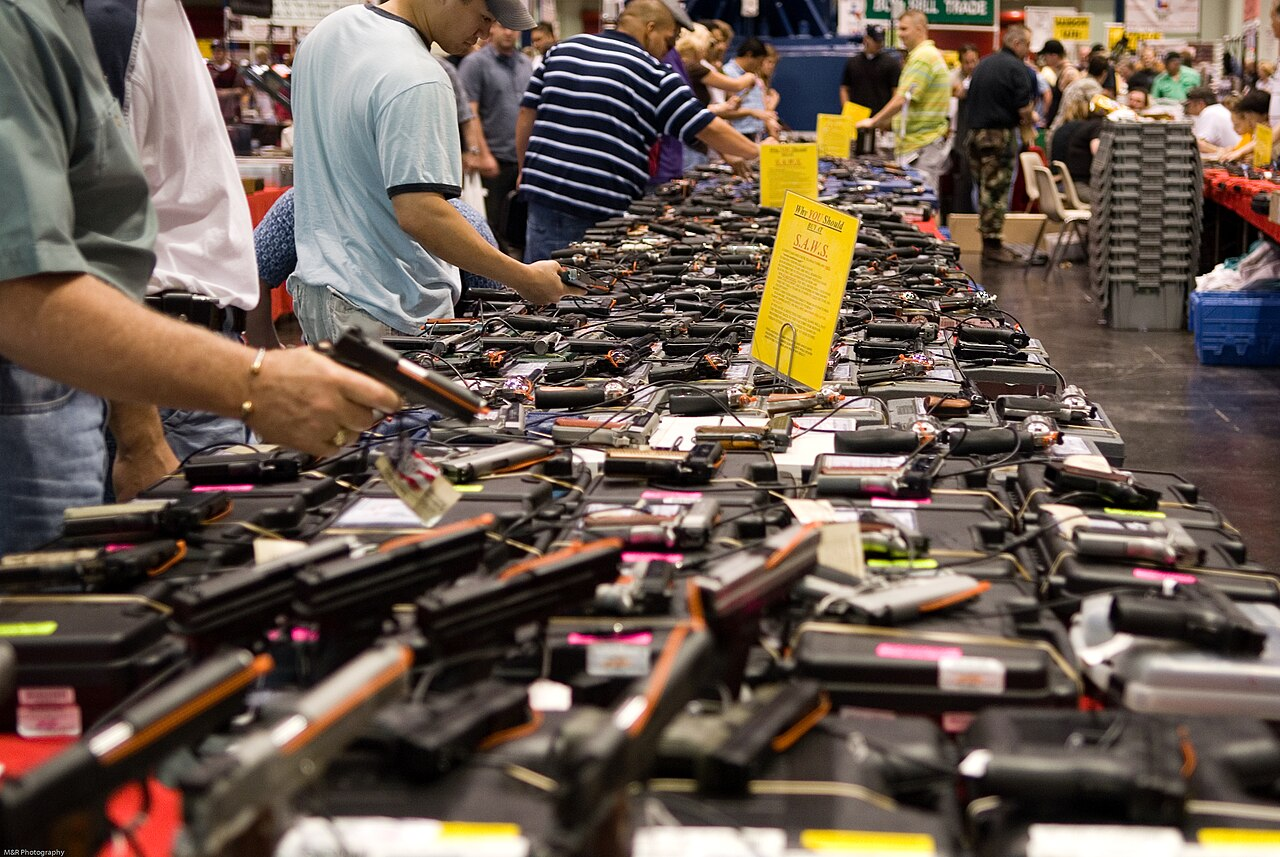
\includegraphics[width=\linewidth]{gunshow.jpg}\\[0.2em]
      {\tiny\color{muted} A gun show in Houston, Texas. Photo: glasgows (Flickr), CC BY 2.0\par}
    \end{column}
  \end{columns}
\end{frame}

% =====================================================================
\section{Gun Culture}

\begin{frame}{Warm-up: how many are there?}
  \begin{itemize}\setlength{\itemsep}{1.2em}
    \item In groups: I'll show you some things that exist in the US
    \item How many of each are there?
    \item \alert{Write down your guess} before each answer
  \end{itemize}
\end{frame}

\guess{McDonald's}{How many McDonald's restaurants are there in the US?}
  {about 13,700}{at the end of 2025}
  {Source: McDonald's, \emph{Restaurants by Market} (2025).}

\guess{Alcohol}{How many bottles of wine's worth of alcohol does the average American drink per year?}
  {about 100 bottles}
  {9.4 liters of pure alcohol, or about 530 drinks, per person aged 14+ (2023)\\[0.3em]
   \color{muted}Austria: about 11.3 liters per person (15+), so roughly 120 bottles}
  {Sources: NIAAA, Surveillance Report \#122 (2025); OECD, \emph{Health at a Glance} (2025). One bottle = 0.75\,l of wine at 12.5\%.}

\guess{Dogs}{How many pet dogs are there in the US?}
  {about 90 million}{in 2024}
  {Source: American Veterinary Medical Association, pet ownership survey (2024).}

\guess{Cars}{How many registered vehicles are there in the US?}
  {about 298 million}{cars, trucks, buses and motorcycles, 2024}
  {Source: Federal Highway Administration, \emph{Highway Statistics} 2024.}

\guess{People}{How many people live in the US?}
  {about 340 million}{}
  {Source: US Census Bureau population estimate.}

\begin{frame}{Now guess: guns}
  \vfill
  \begin{center}
    {\Large How many civilian guns are there\\for every \alert{100 people} in the US?}\\[1.6em]
    {\large\color{muted}Each group: write down one number}
  \end{center}
  \vfill
\end{frame}

\begin{frame}{Civilian guns per 100 people}
  \begin{columns}[c]
    \begin{column}{0.64\textwidth}
      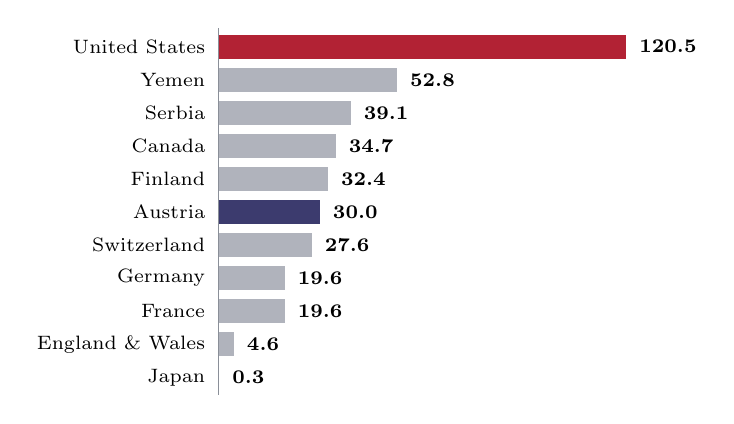
\begin{tikzpicture}[x=0.043cm, y=-0.42cm]
        \foreach \i/\lab/\val/\col in {
            0/United States/120.5/oldred, 1/Yemen/52.8/navy!35, 2/Serbia/39.1/navy!35,
            3/Canada/34.7/navy!35, 4/Finland/32.4/navy!35, 5/Austria/30.0/oldblue,
            6/Switzerland/27.6/navy!35, 7/Germany/19.6/navy!35, 8/France/19.6/navy!35,
            9/England \& Wales/4.6/navy!35, 10/Japan/0.3/navy!35} {
          \fill[\col] (0,\i) rectangle (\val,\i+0.72);
          \node[anchor=east, font=\scriptsize] at (-1,\i+0.36) {\lab};
          \node[anchor=west, font=\scriptsize\bfseries] at (\val+1,\i+0.36) {\val};
        }
        \draw[muted] (0,-0.2) -- (0,10.9);
      \end{tikzpicture}
    \end{column}
    \begin{column}{0.32\textwidth}
      \begin{itemize}\setlength{\itemsep}{0.8em}\small
        \item The US has \alert{more guns than people}
        \item Americans are about 4\% of the world's population\ldots
        \item \ldots but own nearly \alert{half} of its civilian guns (393 of 857 million)
      \end{itemize}
    \end{column}
  \end{columns}
  \source{Source: Small Arms Survey, \emph{Estimating Global Civilian-Held Firearms Numbers} (2018), data for 2017.}
\end{frame}

% =====================================================================
\section{Basic Info}

\begin{frame}{How many guns?}
  \begin{itemize}\setlength{\itemsep}{0.7em}
    \item About \alert{393 million} civilian guns in 2017
    \item Industry-based estimates today: \alert{500 million or more}
    \item More guns than people, but ownership is concentrated:
      \begin{itemize}\setlength{\itemsep}{0.3em}
        \item \textbf{32\%} of adults personally own a gun
        \item About \textbf{4 in 10} live in a household with one
        \item Main reason owners give: \textbf{protection}
      \end{itemize}
  \end{itemize}
  \source{Sources: Small Arms Survey (2018); Pew Research Center, survey of June 2023.}
\end{frame}

\begin{frame}{The Second Amendment (1791)}
  \begin{columns}[c]
    \begin{column}{0.66\textwidth}
      \begin{textquote}
        ``A well regulated Militia, being necessary to the security of a free State, the right of the people to keep and bear Arms, shall not be infringed.''
      \end{textquote}
      \vspace{0.4em}
      \begin{itemize}\setlength{\itemsep}{0.5em}\small
        \item What does it protect? A \alert{militia's} right, or an \alert{individual's} right?
        \item The Supreme Court:
          \begin{itemize}
            \item \emph{Heller} (2008): an individual right to keep a handgun at home
            \item \emph{Bruen} (2022): a right to carry a gun in public; gun laws must fit America's ``historical tradition''
          \end{itemize}
      \end{itemize}
    \end{column}
    \begin{column}{0.28\textwidth}
      \centering
      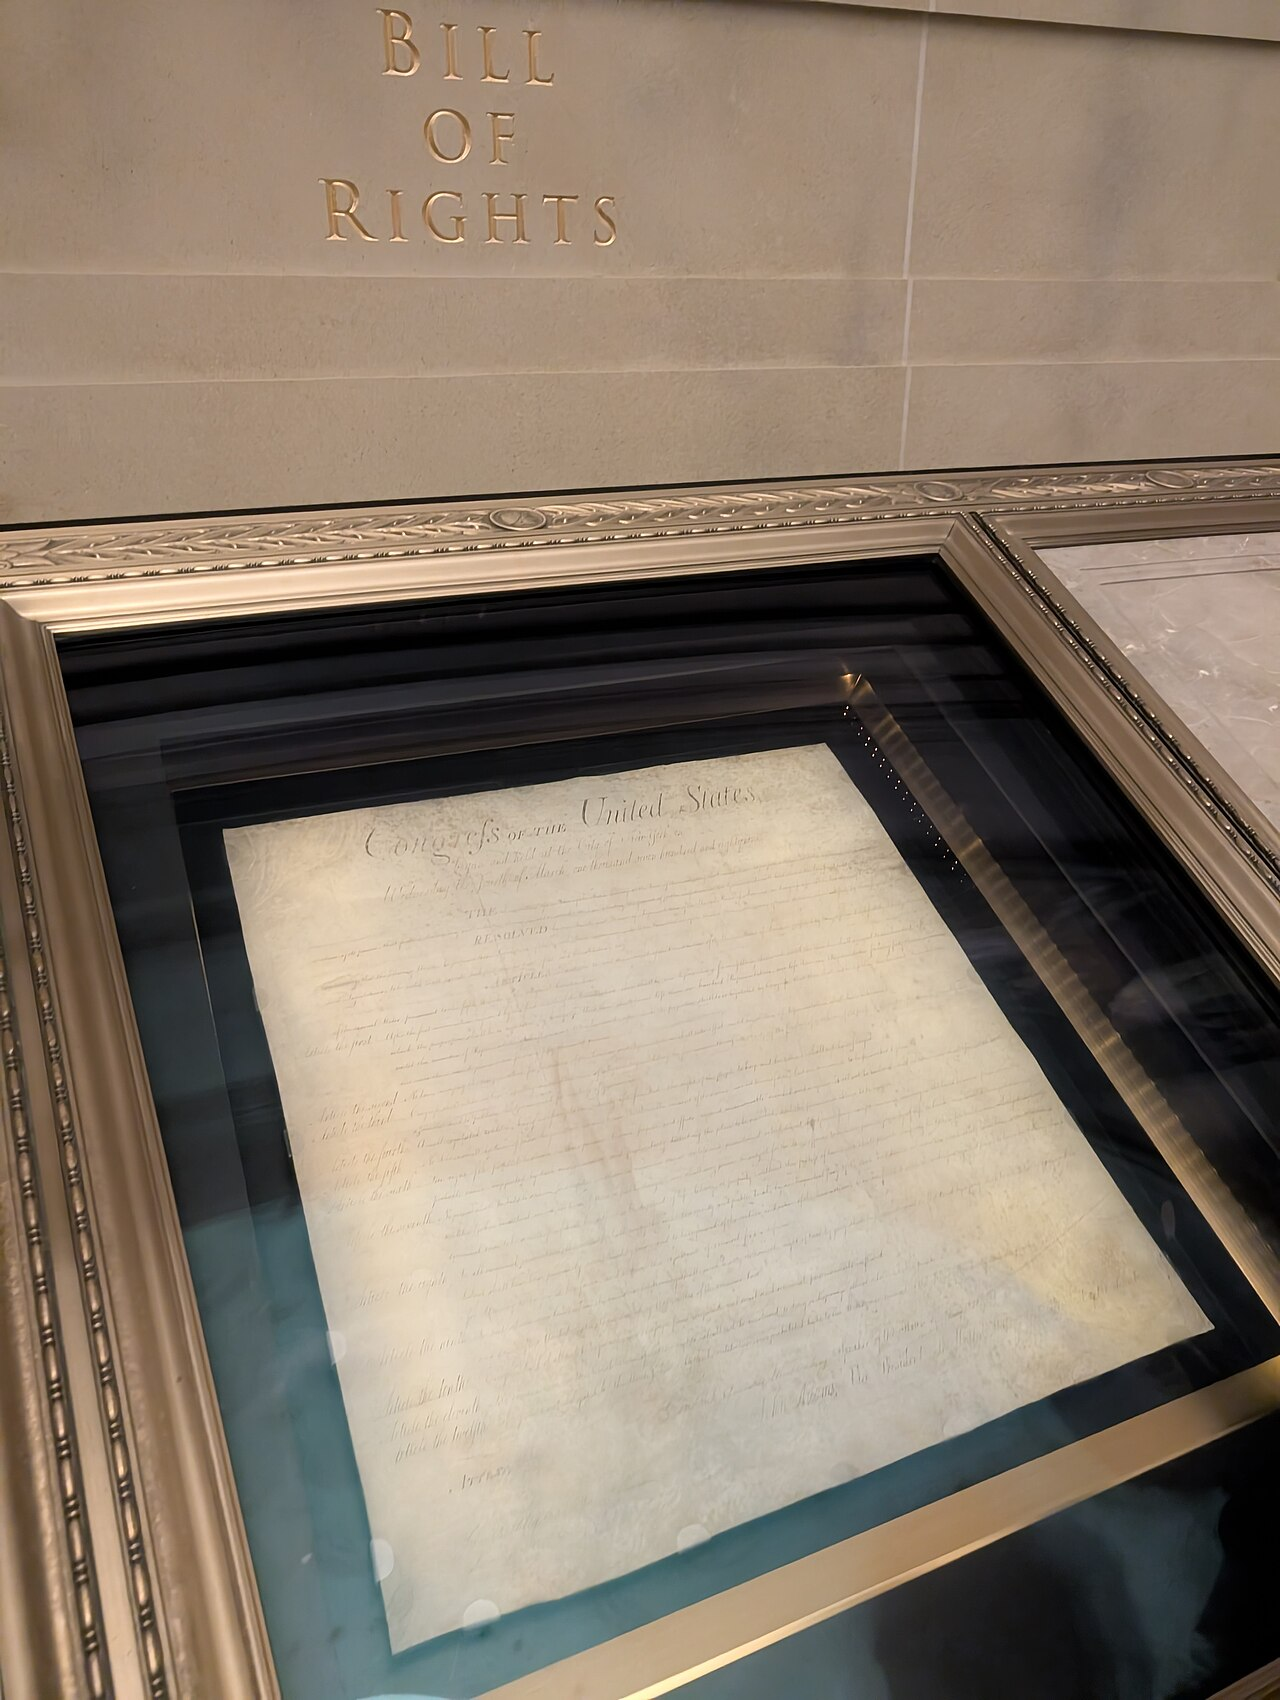
\includegraphics[height=4.6cm]{billofrights.jpg}\\[0.2em]
      {\tiny\color{muted} The Bill of Rights, National Archives. Photo: Runner1928, CC BY-SA 4.0\par}
    \end{column}
  \end{columns}
\end{frame}

\begin{frame}{What's legal, what's not?}
  \begin{itemize}\setlength{\itemsep}{0.9em}
    \item \textbf{Legal nationwide:} handguns, hunting rifles, shotguns, and (in most states) semi-automatic rifles such as the AR-15
    \item \textbf{Nearly impossible:} new fully automatic machine guns. Only those registered before 1986 can be sold to civilians
    \item \textbf{Banned in some states:} ``assault weapons'' and high-capacity magazines (about 10 states + DC, including New York and California)
    \item \textbf{Recently loosened:} the federal tax on silencers and short-barreled rifles dropped to \alert{\$0} in January 2026
  \end{itemize}
\end{frame}

\begin{frame}{Who can buy a gun?}
  \begin{itemize}\setlength{\itemsep}{0.7em}
    \item Licensed dealers must run a \alert{federal background check}, which usually takes minutes
    \item Banned buyers include people convicted of felonies or domestic violence, and people committed to a mental institution
    \item \textbf{Private sales} between individuals: no check needed under federal law; about 20 states require one
    \item Age: \textbf{18} for rifles and shotguns; \textbf{21} for handguns from a dealer (some states set 21 for everything)
    \item \textbf{No federal gun registry} and no federal waiting period
  \end{itemize}
\end{frame}

\begin{frame}{Let's try a background check!}
  \relax{\small\color{muted} Answer \textbf{yes} or \textbf{no}. Simplified from ATF Form 4473, which every buyer at a gun store fills out.\par}
  \vspace{0.5em}
  \begin{columns}[T]
    \begin{column}{0.48\textwidth}
      \begin{enumerate}\setlength{\itemsep}{0.35em}\small
        \item Are you buying this gun \emph{for yourself}, not for someone else?
        \item Are you charged with a felony right now?
        \item Have you ever been convicted of a felony?
        \item Are you running from the police?
        \item Do you use marijuana or other illegal drugs?
      \end{enumerate}
    \end{column}
    \begin{column}{0.48\textwidth}
      \begin{enumerate}\setcounter{enumi}{5}\setlength{\itemsep}{0.35em}\small
        \item Has a court ever found you mentally incompetent, or committed you to a mental institution?
        \item Is there a restraining order against you?
        \item Have you been convicted of domestic violence?
        \item Were you dishonorably discharged from the military?
        \item Are you in the US illegally?
      \end{enumerate}
    \end{column}
  \end{columns}
  \vspace{0.6em}
  \begin{center}
    \small \alert{Yes} to question 1 and \alert{no} to everything else? Then the store calls the FBI\ldots
  \end{center}
\end{frame}

\begin{frame}{The FBI's answer}
  \begin{columns}[T]
    \begin{column}{0.3\textwidth}\centering
      {\fontsize{24}{28}\selectfont\bfseries\color{navy}Proceed}\\[0.4em]
      {\small You can buy the gun\\\color{muted}(the vast majority of checks)}
    \end{column}
    \begin{column}{0.3\textwidth}\centering
      {\fontsize{24}{28}\selectfont\bfseries\color{muted}Delay}\\[0.4em]
      {\small The FBI needs more time\\\color{muted}after 3 business days, the store may sell anyway}
    \end{column}
    \begin{column}{0.3\textwidth}\centering
      {\fontsize{24}{28}\selectfont\bfseries\color{oldred}Deny}\\[0.4em]
      {\small You can't buy the gun}
    \end{column}
  \end{columns}
  \vspace{1.5em}
  \begin{itemize}\setlength{\itemsep}{0.5em}\small
    \item Buyers under 21 get an extra check of juvenile records (since 2022)
    \item Lying on the form is a federal crime
    \item Marijuana: still on the form, but the Supreme Court limited this ban in June 2026 (\emph{US v.\ Hemani})
  \end{itemize}
  \source{Sources: FBI, NICS; ATF Form 4473; Bipartisan Safer Communities Act (2022).}
\end{frame}

\begin{frame}{Carrying a gun in public}
  \begin{itemize}\setlength{\itemsep}{0.9em}
    \item \alert{29 states}: ``permitless'' or ``constitutional'' carry, so no license is needed
    \item Other states require a permit, sometimes with training
    \item Most states also allow \textbf{open carry} (visible, e.g.\ on the hip)
  \end{itemize}
  \source{Source: count as of 2026 (Wikipedia, ``Constitutional carry'').}
\end{frame}

\begin{frame}{Shooting ranges}
  \begin{itemize}\setlength{\itemsep}{0.9em}
    \item Roughly \alert{8,000+} shooting ranges in the US, indoor and outdoor
    \item You can usually \textbf{rent a gun} at the range, often without owning one or having a license
    \item Popular with tourists: Las Vegas ranges advertise machine-gun ``experiences''
  \end{itemize}
  \source{Source: IBISWorld (2025): 8,289 shooting-range businesses.}
\end{frame}

\begin{frame}{Compare: the USA and Austria}
  \small
  \renewcommand{\arraystretch}{1.3}
  \begin{tabular}{@{}>{\raggedright\arraybackslash}p{0.28\textwidth}>{\raggedright\arraybackslash}p{0.29\textwidth}>{\raggedright\arraybackslash}p{0.35\textwidth}@{}}
    \toprule
    & \textbf{\color{oldblue}USA} & \textbf{\color{austria}Austria} \\
    \midrule
    Guns per 100 people & 120.5 & 30.0 \\
    Minimum age, handgun & 21 (from a dealer) & 25 (since 2026) \\
    Minimum age, rifle & 18 & 21 (since 2026) \\
    Psychological test & No & Yes \\
    Waiting period & None federally & 4 weeks for a first gun \\
    Carrying in public & No permit needed in 29 states & \emph{Waffenpass}: only with a proven need, rarely granted \\
    \bottomrule
  \end{tabular}
  \source{Sources: Small Arms Survey (2018); Waffengesetz-Novelle 2025, fully in force since 28 April 2026.}
\end{frame}

% =====================================================================
\section{A Polarized Country}

\begin{frame}[plain]
  \vfill
  \begin{center}
    {\small\color{muted}Key idea}\\[1em]
    {\LARGE\bfseries The U.S. is almost always\\a country of \alert{two minds}.}
  \end{center}
  \vfill
\end{frame}

\begin{frame}{Two Americas}
  \begin{columns}[T]
    \begin{column}{0.47\textwidth}
      \centering
      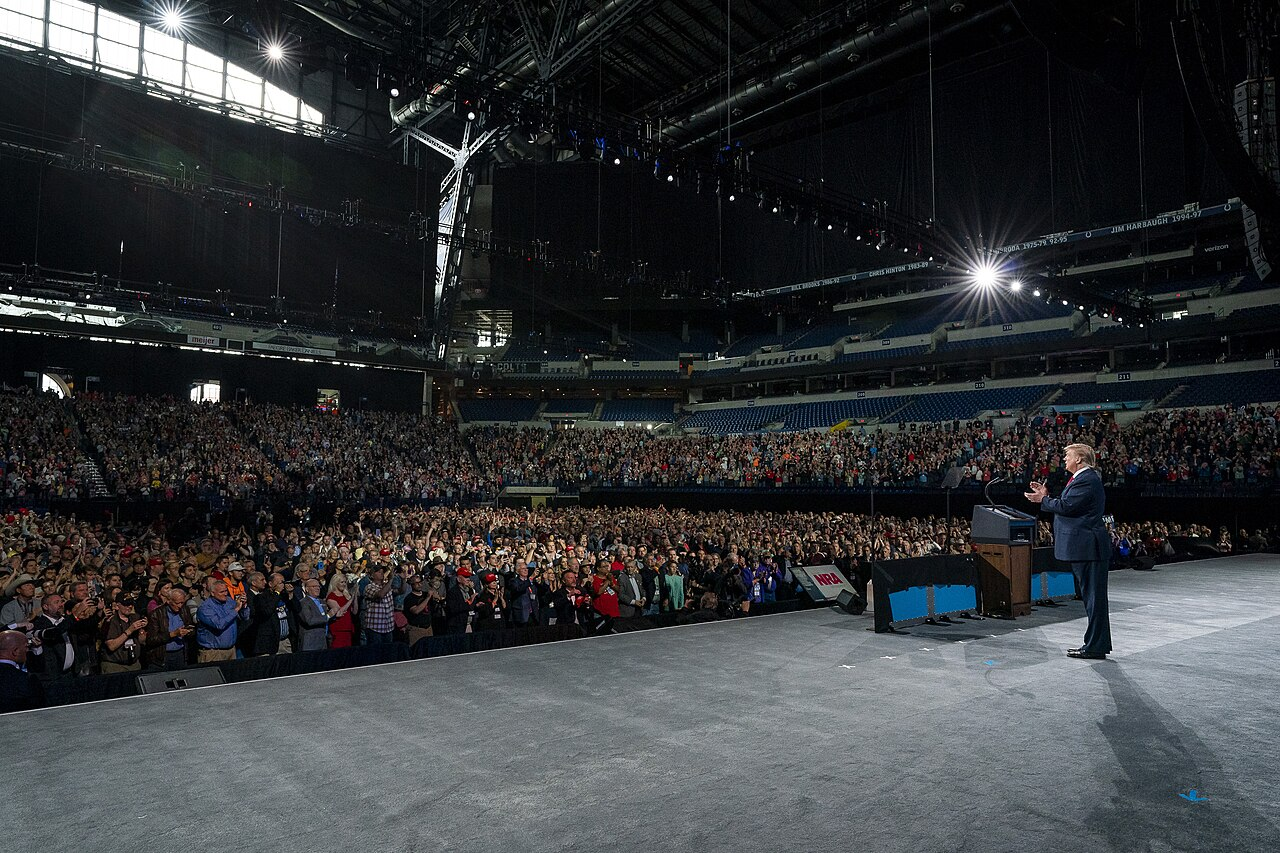
\includegraphics[height=3.6cm]{nra1.jpg}\\[0.2em]
      {\tiny\color{muted} NRA Annual Meeting, Indianapolis, 2019. Photo: The White House, public domain\par}
      \vspace{0.6em}
      {\small Watch: \href{https://www.youtube.com/watch?v=v-qj2rqgChM}{``NRA Conference''}\\
      \color{muted}Channel 5 with Andrew Callaghan\par}
    \end{column}
    \begin{column}{0.47\textwidth}
      \centering
      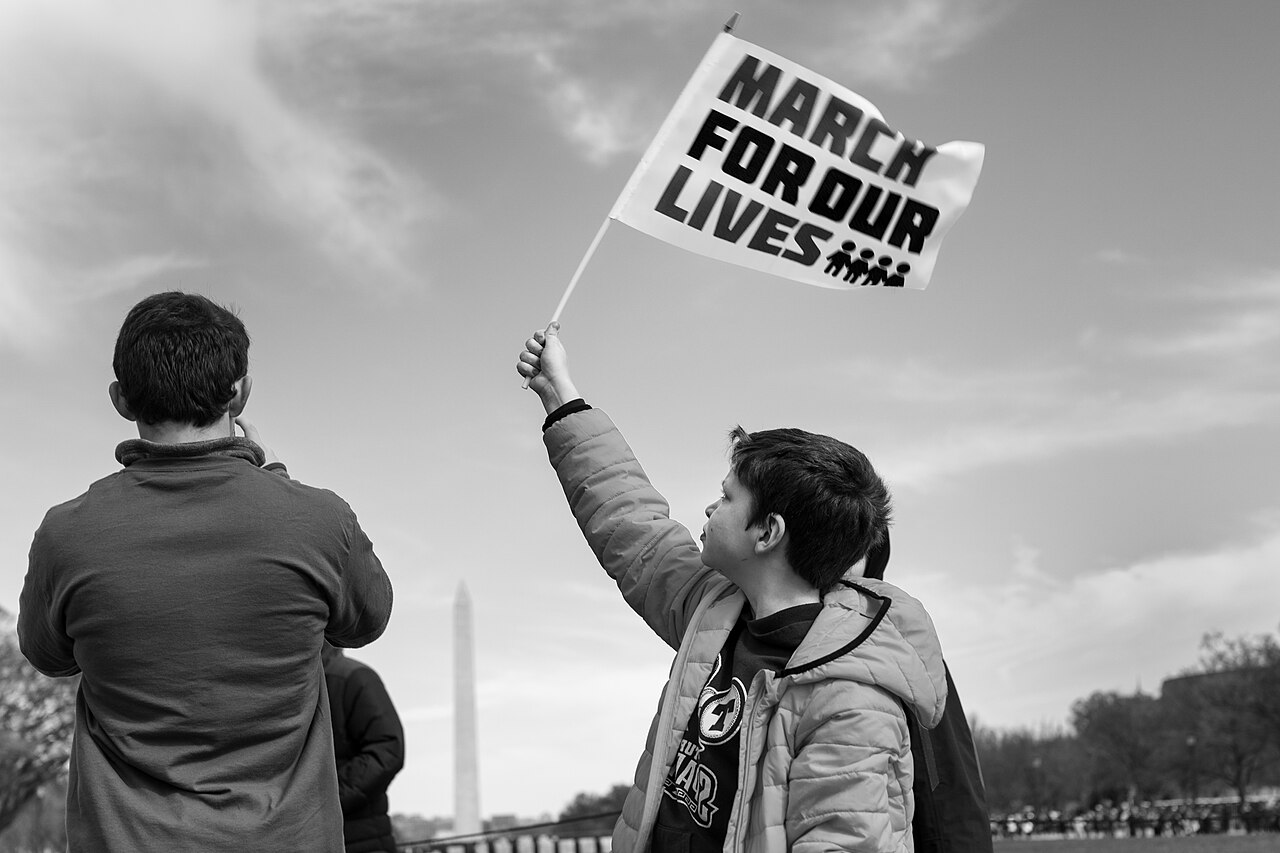
\includegraphics[height=3.6cm]{mfol1.jpg}\\[0.2em]
      {\tiny\color{muted} March for Our Lives, Washington, DC, 2018. Photo: Lorie Shaull, CC BY-SA 2.0\par}
      \vspace{0.6em}
      {\small Watch: \href{https://www.youtube.com/watch?v=IZpvlY6miFM}{``Thousands March to End Gun Violence''}\\
      \color{muted}The New York Times\par}
    \end{column}
  \end{columns}
\end{frame}

\begin{frame}{My experience}
  \begin{columns}[c]
    \begin{column}{0.6\textwidth}
      \begin{itemize}\setlength{\itemsep}{0.6em}\small
        \item I don't know a single person who currently owns a gun
        \item I know only one person (my father) who has ever fired one
        \item At my university, guns were strictly forbidden on campus
          \begin{itemize}
            \item One student was passionate about gun rights, and she was seen as a loser / very weird \raisebox{-0.2em}{
\includegraphics[height=1.2em]{nerd.png}}
          \end{itemize}
        \item But at the \alert{University of Utah} (and other schools), students with a permit can legally carry a concealed gun on campus
      \end{itemize}
    \end{column}
    \begin{column}{0.36\textwidth}
      \centering
      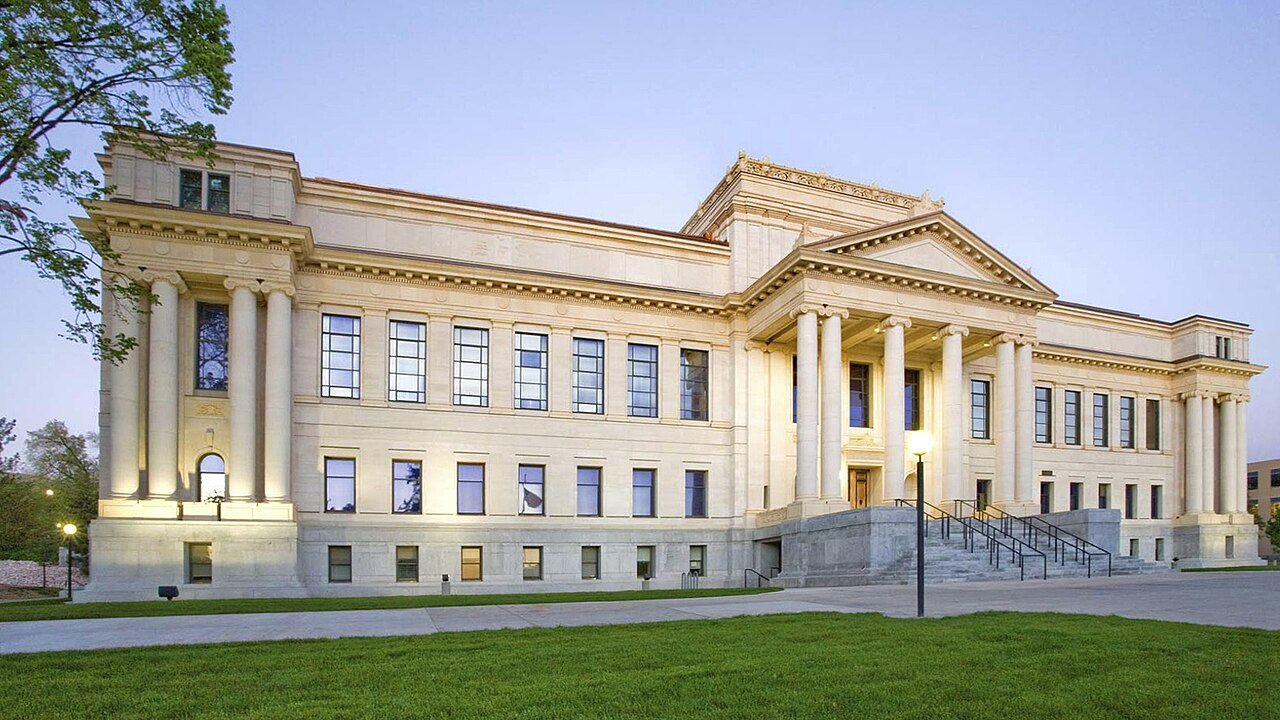
\includegraphics[width=\linewidth]{utah.jpg}\\[0.2em]
      {\tiny\color{muted} Park Building, University of Utah. Photo: University of Utah, CC BY 3.0. Emoji: Google Noto, Apache 2.0\par}
    \end{column}
  \end{columns}
\end{frame}

\begin{frame}{Guns follow party lines}
  \begin{columns}[T]
    \begin{column}{0.48\textwidth}
      \bignum{rep}{45\%}{of Republicans own a gun}
    \end{column}
    \begin{column}{0.48\textwidth}
      \bignum{dem}{20\%}{of Democrats own a gun}
    \end{column}
  \end{columns}
  \vspace{1.2em}
  \begin{itemize}\setlength{\itemsep}{0.5em}\small
    \item Teachers carrying guns at school: \textbf{74\%} of Republicans in favor vs.\ \textbf{27\%} of Democrats
    \item In the Senate, Democrats almost always get an \alert{``F''} from the NRA, Republicans an \alert{``A''}
    \item Last major federal gun law (2022): \textbf{all 50} Democratic senators voted yes, but only \textbf{15 of 50} Republicans
  \end{itemize}
  \source{Sources: Pew Research Center, survey of June 2023; US Senate vote of 23 June 2022.}
\end{frame}

\begin{frame}{New York City: legal, but\ldots}
  \begin{columns}[c]
    \begin{column}{0.62\textwidth}
      \begin{itemize}\setlength{\itemsep}{0.5em}\small
        \item In NYC, \alert{concealed carry is legal} with a license
          \begin{itemize}
            \item i.e.\ you may carry a gun in public, hidden from view
            \item Easier to get since \emph{Bruen} (2022) struck down New York's old ``proper cause'' rule
          \end{itemize}
        \item But the culture strongly tilts against it:
          \begin{itemize}
            \item I've never seen anyone except a police officer carry a gun in the city
            \item If I did, I would panic and probably assume the person was crazy
            \item Carrying is banned on the \textbf{subway}, in \textbf{Times Square}, and in many other ``sensitive places''
          \end{itemize}
      \end{itemize}
    \end{column}
    \begin{column}{0.34\textwidth}
      \centering
      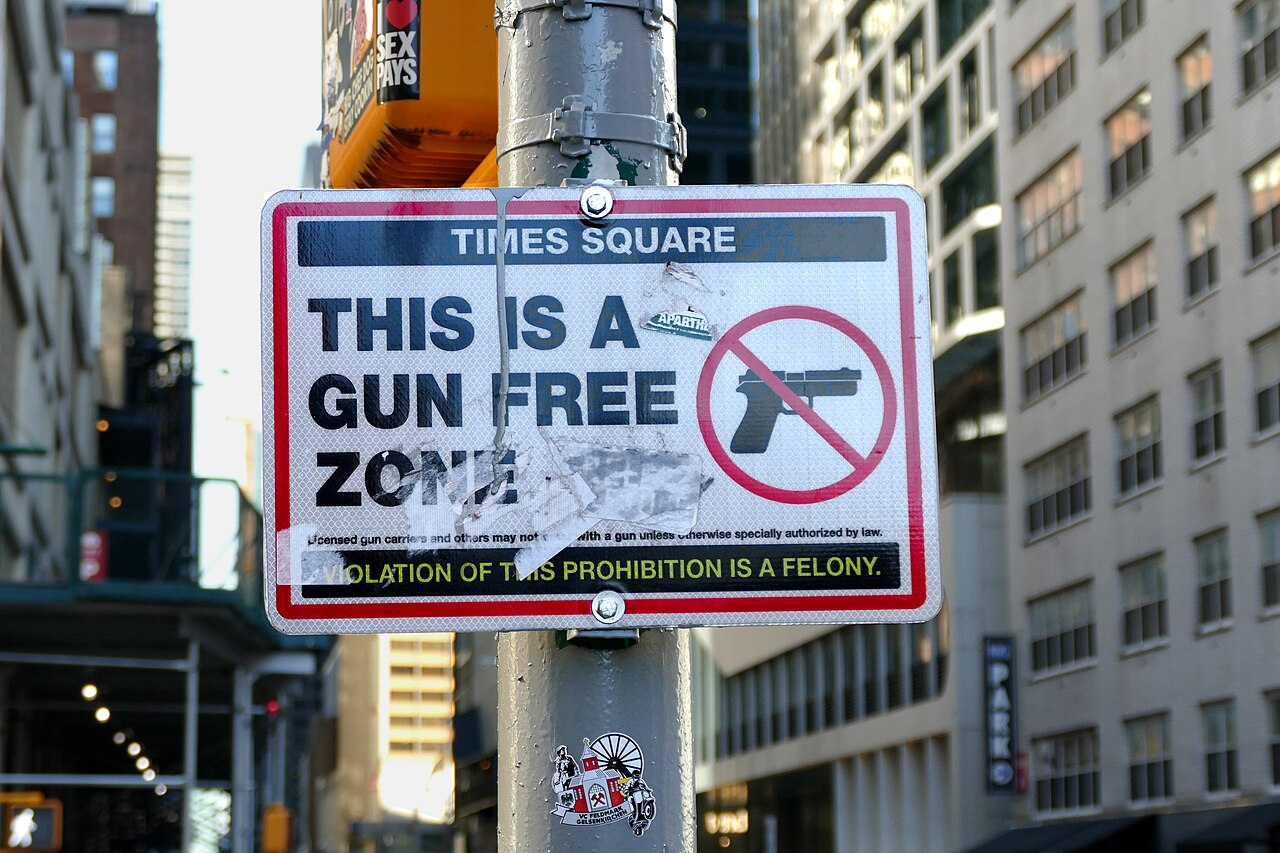
\includegraphics[width=\linewidth]{timessq2.jpg}\\[0.2em]
      {\tiny\color{muted} Times Square. Photo: Kritzolina, CC BY-SA 4.0\par}
    \end{column}
  \end{columns}
\end{frame}

\begin{frame}{Big cities vs.\ everywhere else}
  \begin{itemize}\setlength{\itemsep}{1em}
    \item My impression: it's similar in other big cities
    \item But guns are easy to get almost everywhere:
      \begin{itemize}\setlength{\itemsep}{0.5em}
        \item In most states, an \alert{18-year-old} can legally buy a rifle or shotgun
        \item Handguns from a dealer: usually \alert{21}
      \end{itemize}
  \end{itemize}
\end{frame}

\begin{frame}{Read aloud}
  \relax{\small\color{muted} \emph{The New York Times}, ``American High School Students Are Selling Guns Bound for Cartels,'' 3 October 2026\par}
  \vspace{0.5em}
  \begin{textquote}[fontupper=\itshape\small]
    ``They are too young to buy a beer and barely old enough to drive, yet these four teenage boys have already found their way into the criminal underworld.''\\[0.6em]
    ``On weekends, they drive into the Sonoran Desert outside Phoenix. I watched them line up AR-15s and AK-style rifles against their cars, pose for photos and spend the afternoon shooting targets. At night, they head to parties, smoke pot and scroll endlessly through their social media feeds.''
  \end{textquote}
\end{frame}

\begin{frame}{Read aloud (continued)}
  \relax{\small\color{muted} \emph{The New York Times}, 3 October 2026\par}
  \vspace{0.5em}
  \begin{textquote}[fontupper=\itshape\small]
    ``These teenagers are part of a growing network of American high school students and young adults who are helping to arm some of Mexico's most powerful and violent cartels, according to U.S. officials and trafficking experts who are tracking the trend. They source weapons like handguns and high-caliber rifles, and sell them almost exclusively to cartel operatives based in the United States, the teenagers said.''
  \end{textquote}
  \vfill
  {\scriptsize \href{https://www.nytimes.com/2026/10/03/world/americas/high-school-arms-dealing-mexican-cartels.html?unlocked_article_code=1.NlE.5_Cb.QnFkDBJKkBMg&smid=url-share}{Read the full article (nytimes.com)}\par}
  \vspace{0.6em}
\end{frame}

% =====================================================================
\section{School Shootings}

\begin{frame}{How frequent are they?}
  \begin{itemize}\setlength{\itemsep}{0.8em}
    \item \textbf{2026 so far:} \alert{27} school shootings where someone was hurt or killed\\
      {\small\color{muted}as of 19 October: 17 killed, 29 injured}
    \item Counting \emph{any} gunfire on K-12 and college campuses: \alert{52+}\\
      {\small\color{muted}as of 15 October}
    \item Most school years since 2021 have had \textbf{100+} incidents of gunfire on school grounds
    \item The numbers depend on \alert{how you count}!
  \end{itemize}
  \source{Sources: Education Week school shooting tracker; CNN; Everytown for Gun Safety (144 incidents in 2023--24).}
\end{frame}

\begin{thinkframe}
  {\color{oldred}\textbf{Think}}\\[0.8em]
  How likely is it that an American student\\is shot at school, compared with other dangers?
\end{thinkframe}

\begin{frame}{Putting it in perspective}
  \relax{\small\color{muted} Deaths per year in the US\par}
  \vspace{0.5em}
  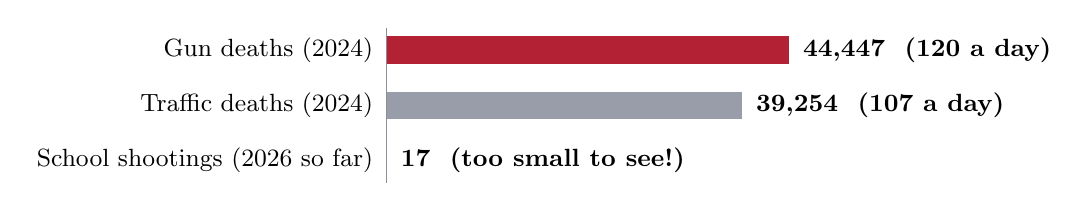
\begin{tikzpicture}[x=0.115cm, y=-0.7cm]
    \foreach \i/\lab/\val/\txt/\col in {
        0/Gun deaths (2024)/44.447/{44,447 \ (120 a day)}/oldred,
        1/Traffic deaths (2024)/39.254/{39,254 \ (107 a day)}/navy!45,
        2/School shootings (2026 so far)/0.017/{17 \ (too small to see!)}/oldblue} {
      \fill[\col] (0,\i) rectangle (\val,\i+0.5);
      \node[anchor=east, font=\small] at (-0.4,\i+0.25) {\lab};
      \node[anchor=west, font=\small\bfseries] at (\val+0.5,\i+0.25) {\txt};
    }
    \draw[muted] (0,-0.15) -- (0,2.65);
  \end{tikzpicture}\\[0.2em]
  {\scriptsize\color{muted} Of all gun deaths: 62\% suicides, 35\% homicides.\par}
  \vspace{0.6em}
  \begin{itemize}\setlength{\itemsep}{0.3em}\small
    \item For any one student, being shot at school is \alert{extremely rare} (about 50 million public school students)
    \item But guns are the \alert{leading cause of death} for American children and teens (ages 1--19), ahead of car crashes, since 2020
  \end{itemize}
  \source{Sources: CDC final 2024 data (via Pew Research Center, 2026); NHTSA; Education Week; CDC WONDER.}
\end{frame}

\begin{frame}{What are we doing about it? (1) Trying to understand it}
  \relax Possible explanations people offer:
  \vspace{0.5em}
  \begin{itemize}\setlength{\itemsep}{0.5em}
    \item Violent video games
    \item Social media
    \item Family dysfunction
    \item Easy access to firearms
    \item Mental illness
  \end{itemize}
  \vspace{0.6em}
  \pause
  \alert{Which of these do you think Americans argue about most? Why?}
\end{frame}

\begin{frame}{What are we doing about it? (2) Arguing about solutions}
  \relax{\small\color{muted} Should laws on gun sales be\ldots{} (Gallup, October 2025)\par}
  \vspace{0.5em}
  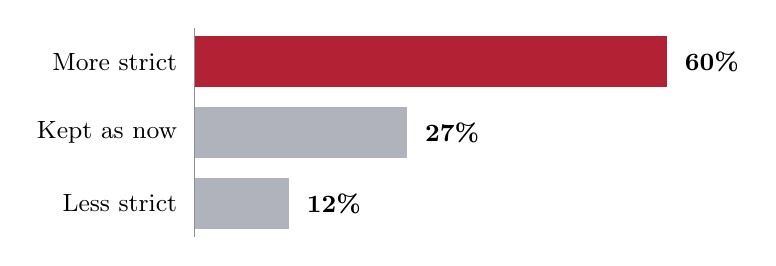
\begin{tikzpicture}[x=0.1cm]
    \foreach \y/\lab/\val/\col in {1.8/More strict/60/oldred, 0.9/Kept as now/27/navy!35, 0/Less strict/12/navy!35} {
      \fill[\col] (0,\y) rectangle (\val,\y+0.65);
      \node[anchor=east, font=\small] at (-1,\y+0.325) {\lab};
      \node[anchor=west, font=\small\bfseries] at (\val+1,\y+0.325) {\val\%};
    }
    \draw[muted] (0,-0.1) -- (0,2.55);
  \end{tikzpicture}
  \vspace{0.6em}
  \begin{itemize}\setlength{\itemsep}{0.4em}\small
    \item \textbf{Almost everyone agrees} on stopping people with mental illness from buying guns: \textbf{\color{rep}88\%} of Republicans, \textbf{\color{dem}89\%} of Democrats
    \item \textbf{Strong disagreement} on banning assault-style weapons: \textbf{\color{dem}85\%} of Democrats in favor; a \textbf{\color{rep}majority} of Republicans opposed
  \end{itemize}
  \source{Sources: Gallup (October 2025); Pew Research Center, survey of June 2023.}
\end{frame}

\begin{frame}{What are we doing about it? (3) Politicians}
  \begin{itemize}\setlength{\itemsep}{0.7em}
    \item \textbf{2022:} Bipartisan Safer Communities Act, the first major federal gun law in about 30 years (after the Uvalde school shooting)
      \begin{itemize}\small
        \item Tougher background checks for buyers under 21; money for ``red flag'' laws and school mental health
      \end{itemize}
    \item \textbf{2025--26:} the Trump administration has loosened federal rules
      \begin{itemize}\small
        \item \$0 tax on silencers; rollback of Biden-era rules on gun-show and private sales
        \item \textbf{Supporters:} restoring Second Amendment rights. \textbf{Critics:} making guns easier to misuse
      \end{itemize}
    \item \textbf{States} are moving in opposite directions: more permitless carry in red states, more restrictions in blue states
  \end{itemize}
\end{frame}

\begin{frame}[plain]
  \vfill
  \begin{center}
    {\LARGE\bfseries\color{navy} How do we think of\\school shootings?}
  \end{center}
  \vfill
\end{frame}

\begin{frame}{Lockdown drills}
  \begin{itemize}\setlength{\itemsep}{1em}
    \item Most American students practice \alert{lockdown drills}: lights off, door locked, hide silently
    \item In 2021--22, about \textbf{96\%} of public schools drilled students on lockdown procedures
    \item Did you ever have drills like this?
  \end{itemize}
  \source{Source: National Center for Education Statistics, Fast Facts.}
\end{frame}

% =====================================================================
\section{Final Activity}

\begin{frame}{Discuss at your tables}
  \vfill
  \begin{center}
    {\Large What might some of the \alert{challenges} be\\in restricting access to guns in the US?}
  \end{center}
  \vfill
  \pause
  \begin{center}
    {\small\color{muted} Think about: the Second Amendment \textbullet{} 400+ million guns already out there \textbullet{} politics \textbullet{} culture}
  \end{center}
  \vspace{1em}
\end{frame}

\begin{frame}{You're in Congress}
  \relax Imagine you are a member of Congress.\\[0.6em]
  Come up with a \alert{piece of legislation} to address gun violence in the U.S.
  \vspace{1em}
  \begin{itemize}\setlength{\itemsep}{0.8em}
    \item What does it do?
    \item Who would support it? Who would oppose it?
    \item Could it pass?
  \end{itemize}
\end{frame}

\end{document}
